%!TEX root = ../thesis.tex
In chapter~\ref{ch:ui} we presented the concept of shape-changing interfaces (SCIs) as


\todo{more introduction, back-reference to chapter 3}

\label{ch:jamming:vocabulary}
In this chapter we will expand our vocabulary regarding SCIs based on \citet{coelho2011shape} and \citet{rasmussen2012shape}.
They both provide contributions as to how we can talk about SCIs, how we can group and identify different types of change of shape, how we can identify and describe shape transformations, and most importantly, how and to which purpose we can interact with SCIs.
We will use this vocabulary onwards in our thesis to discuss SCIs, both ours and others.   

\citeauthor{coelho2011shape} presents a grouping which distinguish three types of change of shape: \emph{topological, textural and permeable} transformations.
Topological transformations here being those transformations which adhere to topological equivalence, permeable those which do not and textural transformation stands as a category for it.
Topologically equivalence here means that a form can transform in to another form by a continuously homeomorphic transformation - that is without cutting or gluing either form.
This can be exemplified by the pliable donut that transforms into a coffee mug without breaking homeomorphism as seen in figure~\ref{pliable-mug} 

\begin{figure}[hb]
	\centering
  		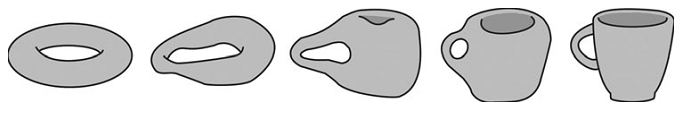
\includegraphics[width=4in]{figures/pliable-donut}
	\caption[The pliable donut momeomorphic transformation, taken from \citep{coelho2011shape}]
   {The pliable donut momeomorphic transformation, taken from \citep{coelho2011shape}}
   \label{pliable-mug}
\end{figure}   
 
\citeauthor{rasmussen2012shape} suggests a grouping more detailed grouping of shape-changing interfaces by identifying eight types of change of shape, namely: \textit{orientation, form, volume, texture, viscosity, spatiality, adding/subtracting and permeability}.
These eight fit into two groups where the first six are topologically equivalent and the last two are not.
This is in line with what \citeauthor{coelho2011shape}, though texture standing has been moved into the topologically equivalent group. Overall it expands on \citeauthor{coelho2011shape}s work and enables us to identify and discuss form changes in more detailed terms.
The grouping is visualized in figure~\ref{types-of-change}, illustrating the different types of change.

\begin{figure}[hb]
	\centering
  		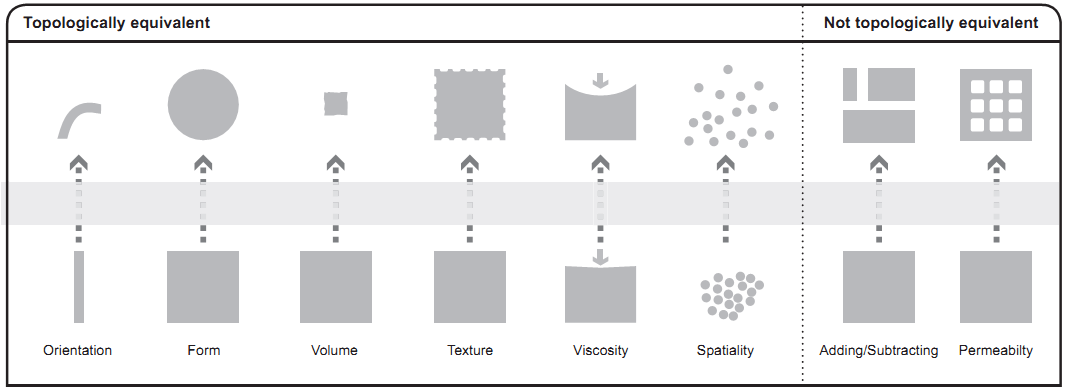
\includegraphics[width=\textwidth]{figures/types-of-change}
	\caption[Types of shape-change as visualised by \citep{rasmussen2012shape}]
   {Types of shape-change as visualised by \citep{rasmussen2012shape}}
   \label{types-of-change}
\end{figure}

There might be some debatable cases in this grouping, e.g. they define textural change as
\begin{quotation}
small changes on the surface of the shape that add visual and tactile properties without affecting the overall form
\end{quotation} 
so if the overall form is not changed it might not make sense to classify it as a homomorphic transformation, which might also be the reason why \citeauthor{coelho2011shape} chose to separate it as a case for itself.
Also if we look at the case of spatiality changes where a collection of elements form a single object, it is possible to think of examples where non-homeomorphic transformations occurs if, for example, the collection of elements split in the middle forming two objects and then merge back together.
This would still count as a shape-changing interface as described in the definition but would not adhere to topological equivalence.   

The transformation in itself is interesting as well and \citeauthor{rasmussen2012shape} identifies different types of transformation.
They describe the transformation as the \textit{phase between endpoints}, meaning the phase between the form's origin and its morphed state.
They distinguish between kinetic parameters and expressive parameters, where the kinetic parameters describe the physical movements of the transformation and the expressive parameters relates to how the kinetic movements are perceived and understood.
This is a very interesting and important aspect of SCIs since it, together with the theory of affordances, provides the basis for understanding the interface and its functions, which at the same time is one of the key challenges of SCIs.
Since SCIs are inherently non-static objects we might not be able to rely on the form alone to communicate the intent and functions of the object. As a change in form can cause a change in function the initial perceived affordance of an objects might not cover all of the interaction possibilities of that object, so there might have to be some interaction clues elsewhere, for example in the transformation itself.

A key aspect of SCIs, and any user interface in general, is the interaction - be it direct physical interaction, implicit visual interaction, or something in between. 
\citeauthor{rasmussen2012shape} distinguish between \textit{no interaction}, where there is only shape-changing output; \textit{indirect interaction}, still only with shape-changing output but based on implicit user input; \textit{direct interaction}, where the user deforms the object in some way as user input and a shape-change output occurs, either in the object itself or in a remote object.
Two approaches to direct interaction are identified, \textit{action and reaction} where the object reacts directly to the action in a synchronized process and \textit{input and output} where the object is acting asynchronously and not necessarily directly related to the input.

In the next session we proceed into the area of jamming, an approach that we see as an interesting enabling technology for SCIs.
Jamming allows for many of the different types of transformations as we will see both in the related jamming applications and in our own concepts. 

Our focus will be on objects with direct interaction and mainly those with input and output merged into the same object, as we here see the best possibilities for creating interfaces \todo{et eller andet}
 
\hl{Our own exploratory work will focus only on topological transformations, excluding spatiality, since our choice of technology hinders this type of change.} This will be further described in section \todo{ref til proto 0}  